%  Typ dokumentu - článek, prezentace aj.
\documentclass[english]{article}

%  Nastaví vstupní a výstupní kódování znaků (encoding) a lokalizace
\usepackage[T1]{fontenc}
\usepackage[utf8]{inputenc}
\usepackage[english,czech]{babel}
\usepackage{icomma}

%  Formát papíru a odsazení od jeho okrajů
\usepackage[letterpaper]{geometry}
\geometry{verbose,tmargin=1.5cm,bmargin=2cm,lmargin=2cm,rmargin=2cm}

%  Umožňuje pracovat s grafikou
\usepackage{graphicx}
\usepackage{bigstrut}
\usepackage{epstopdf}

%  Automaticky odsadí i první paragraf v každé sekci
\usepackage{indentfirst}

%  Umožňuje rozdělovat obsah na více sloupců
\usepackage{multicol}
\usepackage{booktabs}
\usepackage{pgffor}

% physics
\newcommand{\unit}[1]{\ \mathrm{#1}}
\newcommand{\dd}{\mathrm{d}}
\newcommand{\ee}{\mathrm{e}}

%  Umožňuje používat hypertextové odkazy, nastavuje jejich barvu a
%  vlastnosti
\usepackage[unicode]{hyperref}
\hypersetup{
colorlinks=true, citecolor=blue, filecolor=blue, linkcolor=blue,
urlcolor=blue
}

%  Formátování stránek, empty = odstraní číslování
% \pagestyle{empty}

%  Řádkování
\linespread{1.2}

%  Lepší zobrazování matematiky (rozšíření sum o \limits atd.)
\everymath{\displaystyle}
\usepackage{amsmath, amsthm, amssymb}

% Umožní psát přes \mathbb{N/R/Q/..} množiny čísel
\usepackage{amssymb}

%  Velikost fontu matematických výrazů v dokumentu lze pro danou
% základního fontu dokumentu upravit pomocí:
% \DeclareMathSizes{X}{Y}{Z}{U} kde:
% X je velikost fontu v dokumentu, pro kterou se matematika upraví
% Y je standartní velikost fontu matematiky
% Z je velikost fontu zmenšených (vnořených výrazů)
% U je velikost fontu ještě více zmenšených (vnořených výrazů).
\DeclareMathSizes{10}{10.5}{9}{9}

%  Nastaví autora, název, datum, skupinu měření apod. (můj vlastní
% příkaz, umožní znovu-použití v dokumentu)
\newcommand{\Author}{David Roesel}
\newcommand{\Coauthor}{Tereza Schönfeldová}
\newcommand{\Institute}{FJFI ČVUT v Praze}
\newcommand{\Subject}{FYZIKÁLNÍ PRAKTIKUM II}
\newcommand{\Group}{7}
\newcommand{\Circle}{ZS 7}
\newcommand{\Title}{Úloha \#4  \\Balmerova série}
\newcommand{\Date}{28.4.2014}

% Začátek dokumentu - Formátování na výstup
\begin{document}

% Interní proměnné, možno zobrazovat u prezentací, používají se při
% generování pomocí \titlepage apod.
\author{\Author}
\title{\Title}
\date{\Date}

%  Lokalizace některých názvů do češtiny
\renewcommand{\figurename}{Obr.}
\renewcommand{\tablename}{Tab.}
\renewcommand{\refname}{Reference}

% --- Hlavička dokumentu -----------------------------------------------

\setlength{\parindent}{0cm}
\begin{multicols}{2}
\textbf{\Subject \\
        \Institute \\[0.1cm]
%\large  \Title \\[0.5cm]
\Title \\[0.5cm]
}
\begin{tabular}{rlrl}
\large Datum měření: & \Date & \large Skupina: & \Group \\
\large Jméno: & \Author & \large Kroužek:  & \Circle\\
\large Spolupracovala: & \Coauthor &\large Klasifikace:\\
\end{tabular}

\begin{flushright}

\includegraphics[scale=0.28]{../../_meta/fjfi_standart.pdf}
\hspace{0.2cm}

\includegraphics[scale=0.28]{../../_meta/cvut_standart.pdf}
\end{flushright}
\end{multicols}
\hrule
\vspace{0.5cm}

% ----------------------------------------------------------------------


% --- Tělo dokumentu ---------------------------------------------------
\setlength{\parindent}{0.5cm}
\section{Pracovní úkoly}
\begin{enumerate}
\item \textbf{(Nepovinné)} V přípravě nalezněte obecně pro $\alpha_1 \neq \alpha_2$ podmínku nejmenší deviace $\alpha_1=\alpha_2$ a z toho odvoďte vzorec (12) v zadání \cite{bib:zadani}.

\textbf{Návod:} Uvědomte si, že deviace $\varepsilon$ je složenou funkcí $\alpha_1:\varepsilon=\varepsilon(\alpha_2(\beta_2(\beta_1(\alpha_1))))$

\item V přípravě odvoďte vzorec (12) v zadání \cite{bib:zadani} v případě, že je splněna podmínka nejmenší deviace $\alpha_1=\alpha_2$.

\item V přípravě vypočtěte (i numericky) hodnotu Rydbergovy konstanty (tj. odvoďte vztah (11) ze vztahů (6), (10) a (9) v zadání \cite{bib:zadani}).

\item V přípravě odvoďte vzorce (14) a (17) ze zadání \cite{bib:zadani}.

\item Metodou dělených svazků změřte lámavý úhel hranolu. Měření proveďte 5x.

\item Změřte index lomu hranolu v závislosti na vlnové délce pro čáry rtuťového spektra, nakreslete graf a fitováním nelineární funkcní (13) z \cite{bib:zadani} určete disperzní vztah $n=n(\lambda)$.

\item Změřte spektrum vodíkové výbojky (Balmerovu sérii atomu vodíku) a ověřte platnost vztahu (3) z \cite{bib:zadani}.

\item Metodou nejmenších čtverců nebo fitováním spočtěte Rydbergovu konstantu pro atomární vodík. Výpočet této konstanty je analogický jako výpočet Planckovy konstanty v úloze Studium rentgenového spektra Mo anody. Podívejte se na úkol č. 4 této úlohy.

\item Určete charaktesristickou disperzi $\mathrm{d}n/\mathrm{d}\lambda$ v okolí vlnové délky 589 nm (žluté čáry v sodíkovém spektru).

\item Určete rozlišovací schopnost hranolu pro sodíkový dublet a vypočítejte minimální velikost základny hranolu, vyrobeného ze stejného materiálu jako hranol, s kterým měříte, který je ještě schopen rozlišit sodíkový dublet.

\end{enumerate}

	
\section{Vypracování}

	\subsection{Použité přístroje}
		Goniometr, kolimátor, dalekohled, rtuťová, sodíková a vodíková výbojka, hranol, mobilní telefon, lupa.
	
	\subsection{Teoretický úvod}
		
		\subsubsection{Úhel nejmenší deviace}
			Při měření úhlu nejmenší deviace $\varepsilon_0$ vycházíme ze vzorce 		
			\begin{equation}
			\varepsilon_0=\frac{|\alpha_1-\alpha_2|}{2},
			\label{eq:deviace}
			\end{equation}
			kde $\alpha_1$ a $\alpha_2$ jsou úhly, které pro danou spektrální čáru odečteme z goniometru (a to v obou zrcadlových sestaveních experimentu). Pro detailní odvození viz domácí příprava.
			
		\subsection{Index lomu}
			Platí-li podmínka nejmenší deviace $\varepsilon_0$, můžeme relativní index lomu spočítat pomocí vztahu
			\begin{equation}
			n=\frac{\sin\left(\frac{\varepsilon_0+\varphi}{2}\right)}{\sin\left(\varphi / 2\right)},
			\label{eq:index_lomu}
			\end{equation}
			
			kde $\varepsilon_0$ je úhel nejmenší deviace a $\varphi$ je lámavý úhel hranolu. Pro detailní odvození viz domácí příprava.
			
		\subsubsection{Spektrální série energetických hladin atomu vodíku}
			Během studia spektrálních čar atomistického vodíku bylo v roce 1885 zjištěno, že pro vlnové délky čtyř čar jeho spektra označených $H_{\alpha, \beta, \gamma, \delta}$ jdou jejich hodnoty vyjádřit empirickým vztahem 
			\begin{equation}
				\lambda = B\frac{n^2}{n^2-4},\qquad n=3,4,5,6, \qquad B=364,56~\unit{mm}.
			\end{equation}
			
			Vlnové délky $\lambda$ spektrálních čar lze pro atomární vodík ve viditelném spektru vyjádřit podle vztahu 
			\begin{equation}
			\frac{1}{\lambda}=\frac{4}{B}\left( \frac{1}{2^2}-\frac{1}{n^2}\right),
			\label{eq:balmerova serie vodik}
			\end{equation}
			kde $4/B=R$, což je tzv. \emph{Rydbergova konstanta}.
		
		\subsubsection{Disperzní závislost}
			Průběh disperzní závislosti jde aproximovat různými vzorci. My budeme využívat následujícího vztahu
			\begin{equation}
			n=n_n+\frac{C}{\lambda-\lambda_n},
			\label{eq:disperzni zavislost}
			\end{equation}
			kde $n_n$, $C$ a $\lambda_n$ jsou konstanty, které určíme lineární regresí této funkce z naměřených dat.
		
		\subsection{Rozlišovací schopnost hranolu}
			Uvažujme rovnoramenný hranol. Rozlišovací schopnost je přímo ovlivňována ohybovými jevy, které nastávají při průchodu světla hranolem. Obvykle tuto schopnost charakterizujeme veličinou 
			\begin{equation}
				R=\frac{\lambda}{\Delta\lambda},
				\label{rzl_1}
			\end{equation}
			kde $\Delta\lambda$ je minimální diference vlnových délek, které ještě mohou být hranolem rozlišeny. Z odvození v domácí přípravě přímo plyne, že pro náš případ (za uvažování svazku rovnoběžných paprsků a dodržení podmínky pro minimální deviaci) platí 
			\begin{equation}
				R=a\frac{\dd n}{\dd \lambda},
				\label{rzl_2}
			\end{equation}
			kde $a$ je délka $|BC|$ z Obr.~4 v \cite{bib:zadani}.
				
	\subsection{Postup měření}
		\subsubsection{Lámavý úhel hranolu}
			Nejprve jsme chtěli změřit lámavý úhel hranolu $\varphi$, který potřebujeme pro zpracování všech následujících měření. Stolek s hranolem jsme nastavili tak, aby světlo dopadalo téměř přímo na hranu hranolu, tedy aby docházelo k odrazu a ne k lomu světla. Následně jsme použili kolimátor tak, aby na hranol dopadalo světlo pouze v podobě úzkého proužku, který jsme poté hledali v dalekohledu. Pomocí goniometru jsme následně změřili úhel mezi oběma obrazy a jeho polovina nám udávala lámavý úhel $\varphi$.
		
		\subsubsection{Úhel minimální deviace}
			Před štěrbinu kolimátoru jsme umístili daný zdroj světla (např. rtuťovou výbojku) a nastavili jsme hranol tak, aby docházelo k lomu světla. V dalekohledu jsme následně hledali spektrální čáry a porovnávali je s teoretickou podobou spektra přímo u úlohy. Za otáčení stolku i dalekohledu jsme následně hledali moment, kdy se spektrální čáry přestanou pohybovat jedním směrem a začnou putovat směrem druhým. V momentu tohoto zastavení spektrálních čar jsme odečetli úhel na goniometru pro každou z nich. Postup jsme opakovali taktéž pro druhou lámavou hranu našeho hranolu. 
		
	\subsection{Naměřené hodnoty}
		\subsubsection{Lámavý úhel hranolu}
			Naměřené hodnoty pro výpočet lámavého úhlu hranolu jsou uvedeny v Tab.~\ref{tab:lamavy_uhel}. Hodnotu tohoto úhlu jsme pro každé měření určili jako polovinu rozdílu úhlů obou odrazů a finální hodnotu lámavého úhlu jsme spočítali jako aritmetický průměr našich měření (\ref{eq:aritmeticky_prumer}) s chybou podle (\ref{eq:chyba_aritmetickeho_prumeru}) a finální hodnotou 
			\begin{equation}
				\varphi = (60,05\pm0,02)^\circ.
			\end{equation}
			
			% Table generated by Excel2LaTeX from sheet 'List1'
			\begin{table}[htbp]
			  \centering
			    % Table generated by Excel2LaTeX from sheet 'List1'
    \begin{tabular}{|r|r|r|}
    \hline
    \boldmath{}\textbf{$\varphi_1~\unit{[^\circ]}$}\unboldmath{} & \boldmath{}\textbf{$\varphi_2~\unit{[^\circ]}$}\unboldmath{} & \boldmath{}\textbf{$\varphi~\unit{[^\circ]}$}\unboldmath{} \bigstrut\\
    \hline
    41,42 & 281,13 & 60,14 \bigstrut\\
    \hline
    37,72 & 277,62 & 60,05 \bigstrut\\
    \hline
    40,80 & 280,75 & 60,03 \bigstrut\\
    \hline
    39,62 & 279,62 & 60,00 \bigstrut\\
    \hline
    46,48 & 286,42 & 60,03 \bigstrut\\
    \hline
    \end{tabular}%

			    
			      \caption{Naměřené hodnoty pro výpočet lámavého úhlu hranolu; $\varphi_1$ a $\varphi_2$ jsou úhly obou obrazů určené s chybou $0,02^\circ$, $\varphi$ je pak z nich vypočítaná hodnota lámavého úhlu pro každé měření.}
			  \label{tab:lamavy_uhel}%
			\end{table}%
			
		
		\subsubsection{Index lomu pro čáry rtuťového spektra}
			Naměřené hodnoty pro výpočet úhlu minimální deviace (\ref{eq:deviace}) a tím i indexu lomu (\ref{eq:index_lomu}) pro každou ze spektrálních čar rtuťového spektra jsou uvedeny v Tab.~\ref{tab:hg} s chybami určenými podle (\ref{eq:chyba_neprime_mereni}). Naměřené hodnoty jsou také vyneseny do grafu na Obr.~\ref{fig:g_hg}. Disperzní vztah jsme určili jako 
			\begin{equation}
				n(\lambda)=(1,508\pm0,002)+\frac{(3\pm1)}{\lambda-(273\pm30)}~\unit{[-]}.
				\label{eq:disperzni_vztah}
			\end{equation}
			
			% Table generated by Excel2LaTeX from sheet 'List1'
			\begin{table}[htbp]
			  \centering
    \begin{tabular}{|r|r|r|r|r|}
    \hline
    \boldmath{}\textbf{$\lambda~\unit{[nm]}$}\unboldmath{} & \boldmath{}\textbf{$d_1~\unit{[^\circ]}$}\unboldmath{} & \boldmath{}\textbf{$d_2~\unit{[^\circ]}$}\unboldmath{} & \boldmath{}\textbf{$\varepsilon_0~\unit{[^\circ]}$}\unboldmath{} & \boldmath{}\textbf{$n~\unit{[-]}$}\unboldmath{} \bigstrut\\
    \hline
    690,7 & 26,63 & 309,40 & 38,62 & 1,5159 \bigstrut\\
    \hline
    579,1 & 26,77 & 309,22 & 38,78 & 1,5177 \bigstrut\\
    \hline
    546,1 & 26,88 & 309,10 & 38,89 & 1,5190 \bigstrut\\
    \hline
    491,6 & 27,15 & 308,80 & 39,18 & 1,5222 \bigstrut\\
    \hline
    435,8 & 27,60 & 308,32 & 39,64 & 1,5275 \bigstrut\\
    \hline
    407,8 & 27,82 & 308,00 & 39,91 & 1,5305 \bigstrut\\
    \hline
    \end{tabular}%

			    \caption{Naměřené a vypočítané hodnoty pro spektrum $Hg$; $\lambda$ je vlnová délka dané spektrální čáry \cite{bib:na_miste}, $d_1$ a $d_2$ jsou úhly obou odrazů určené s chybou $0,02^\circ$, $\varepsilon_0$ je z nich spočítaný úhel nejmenší deviace (\ref{eq:deviace}) s chybou $0,01^\circ$ (\ref{eq:chyba_neprime_mereni}) a $n$ index lomu pro danou spektrální čáru vypočítaný podle (\ref{eq:index_lomu}) s chybou všech měření (po zaokrouhlení) $0,0003$ (\ref{eq:chyba_neprime_mereni}).}
			  \label{tab:hg}%
			\end{table}%
			
		\subsubsection{Spektrum vodíkové výbojky}
			Naměřené hodnoty pro spektrum vodíkové výbojky jsou vyneseny v Tab.~\ref{tab:h2}. Hodnoty vlnových délek, vypočítané z nich podle předchozího vztahu s chybou podle (\ref{eq:chyba_neprime_mereni}), jsou následně vyneseny do grafu na Obr.~\ref{fig:g_r} a proloženy za účelem výpočtu Rydbergovy konstanty pro atomický vodík, kterou jsme určili jako
			\begin{equation}
				R = ( 0,0108\pm0,0003 )~\unit{ nm^{-1} }.
			\end{equation}
		
			% Table generated by Excel2LaTeX from sheet 'List1'
			\begin{table}[htbp]
			  \centering
    \begin{tabular}{|r|r|r|r|r|r|r|}
    \hline
    \boldmath{}\textbf{$\lambda~\unit{[nm]}$}\unboldmath{} & \boldmath{}\textbf{$d_1~\unit{[^\circ]}$}\unboldmath{} & \boldmath{}\textbf{$d_2~\unit{[^\circ]}$}\unboldmath{} & \boldmath{}\textbf{$\varepsilon_0~\unit{[^\circ]}$}\unboldmath{} & \boldmath{}\textbf{$n~\unit{[-]}$}\unboldmath{} & \boldmath{}\textbf{$n_{t}~\unit{[-]}$}\unboldmath{} & \boldmath{}\textbf{$\sigma_{n_{t}}~\unit{[-]}$}\unboldmath{} \bigstrut\\
    \hline
    656,3 & 26,28 & 309,17 & 38,56 & 1,5152 & 1,5   & 0,2 \bigstrut\\
    \hline
    486,1 & 27,00 & 308,67 & 39,17 & 1,5221 & 1,5   & 0,4 \bigstrut\\
    \hline
    434,0 & 27,72 & 308,18 & 39,77 & 1,5289 & 1,5   & 0,6 \bigstrut\\
    \hline
    \end{tabular}%

			    \caption{Naměřené a vypočítané hodnoty pro spektrum $H_2$; $\lambda$ je vlnová délka dané spektrální čáry \cite{bib:na_miste}, $d_1$ a $d_2$ jsou úhly obou odrazů určené s chybou $0,02^\circ$, $\varepsilon_0$ je z nich spočítaný úhel nejmenší deviace (\ref{eq:deviace}) s chybou $0,01^\circ$ (\ref{eq:chyba_neprime_mereni}), $n$ index lomu pro danou spektrální čáru vypočítaný podle (\ref{eq:index_lomu}) s chybou všech měření (po zaokrouhlení) $0,0003$ (\ref{eq:chyba_neprime_mereni}) a $n_t$, $\sigma_{n_t}$ je teoretické hodnota indexu lomu spočítaná pomocí disperzního vztahu (\ref{eq:disperzni_vztah}) i se svou chybou (\ref{eq:chyba_neprime_mereni}).}
			  \label{tab:h2}%
			\end{table}%		
		
		\subsubsection{Sodíkové spektrum}
			Charakteristickou disperzi jsme určili zderivováním vztahu (\ref{eq:index_lomu}) a následným dosazením vlnové délky $\lambda = 589~\unit{nm}$ a parametrů fitu získaných pro rtuťové spektrum. Tímto postupem jsme získali hodnotu charakteristické disperze v okolí žluté čáry v sodíkovém spektru jako
			\begin{equation}
				\frac{\dd n}{\dd \lambda} = ( 3 \pm 1 )\unit{\cdot 10^5~[-]}.
			\end{equation}
		
		\subsubsection{Rozlišovací schopnost hranolu}
			Z údajů u úlohy plynulo, že bychom sodíkový dublet měli pozorovat na vlnových délkách 588,9 a 589,6~nm. Rozlišovací schopnost jsme určili podle vztahu (\ref{rzl_1}) za použití $\lambda=(589,3\pm0,4)\unit{~nm}$ (aritmetického průměru těchto délek) s chybou podle (\ref{eq:chyba_neprime_mereni}) jako
			\begin{equation}
				R_{Na} = ( 841,8 \pm 0,5 )~\unit{[-]}.
			\end{equation}
			
			Z této hodnoty následně můžeme také vypočítat, jak velký by musel být hranol, abychom pomocí něj mohli sodíkový dublet pozorovat. Délku hranolu $a$ jsme spočítali podle vztahu (\ref{rzl_2})  s chybou podle (\ref{eq:chyba_neprime_mereni}) a určili jsme její hodnotu na
			\begin{equation}
				a = (3 \pm 1) ~\unit{cm}.
			\end{equation}
		
	\subsection{Diskuse}
		Už při měření lámavého úhlu $\varphi$ bylo jasné, že určení úhlu je méně přesné, než nejmenší dílek měřítka. U všech měření počítáme s chybou $0,02^\circ$, ale dalekohled nebylo snadné umístit přesně do středu proužku (nebo na rozhraní barev spektra v dalších úlohách) a vznikala tak větší chyba než několik dílků měřítka.
		
		Uváděné úhly jsou přímo hodnoty odečtené z měřítka. Pro výpočty bylo potřeba přičíst ke druhému úhlu $360^\circ$ jako korekci za použité měřítko. Odečítání úhlů z měřítka bylo také zkomplikované špatnými světelnými podmínkami v místnosti a tím jak výrazně se stupnice leskla.
		
		Index lomu pro čáry rtuťového spektra se nám podařilo určit úspěšně a pozorovali jsme každou z teoreticky předpokládaných \cite{bib:na_miste}. Naměřené hodnoty se nám následně podařilo také rozumně nafitovat a získat tak kýženou závislost. Závislost by šlo zpřesnit hledáním více známých pozic ve spektru, ale parametry by to pravděpodobně příliš neovlivnilo (maximálně by to zmenšilo jejich předpokládanou chybu).
		
		Při proměřování spektra vodíkové výbojky se nám bohužel podařilo nalézt pouze tři ze čtyř předpokládaných spektrálních čar (viděli jsme modrou, ale fialovou už se nám nepodařilo rozpoznat). Při tomto měření mohlo dojít, vzhledem k odchylce od tabulkové hodnoty, k chybnému odečtení úhlu z goniometru. Měření by se dalo zlepšit naměřením úhlů vícekrát, případně použitím většího počtu definovaných (a viditelných) čar spektra.
		
		Tyto hodnoty jsme i tak vynesli do grafu a proložili je závislostí pro zjištění Rydbergovy konstanty. I přes nepřesně změřené hodnoty a jejich malý počet nám k parametru fitu $R$ program \emph{GNUplot} určil relativně nízkou hodnotu chyby. Hodnota Rydbergovy konstanty nám vyšla $R = ( 0,0108\pm0,0003 )~\unit{ nm^{-1} }$, což je velice blízko v domácí přípravě odvozené hodnotě  $R = 0,0110~\unit{ nm^{-1} }$, i když se tato teoretická hodnota jen těsně dotýká chybového intervalu určeného fitem. Celkově můžeme říct, že závislost odpovídá našim hodnotám a že se nám vztah podařilo ověřit úspěšně.
		
		Sodíkový dublet se nám s naším hranolem rozlišit nepodařilo. Vypočítali jsme, že minimální velikost hranolu pro rozlišení dubletu by odpovídala délce stěny $a=(3\pm1)~\unit{cm}$, což přímo nezaručuje, že by to s naším hranolem jít muselo. Kromě rozměru hranolu však naši schopnost rozlišení dubletu pravděpodobně ovlivňovala také velikost štěrbiny kolimátoru, špatné světelné podmínky v místnosti, případně jiné nedokonalosti našich pozorovacích prostředků. S větším hranolem by však byla pravděpodobnost rozlišení dubletu o poznání větší.
		
\section{Závěr}
	V přípravě jsme odvodili vzorec (12) z \cite{bib:zadani} pro splněnou podmínku $\alpha_1=\alpha_2$. Tamtéž jsme vypočetli (i numericky) hodnotu Rydbergovy konstanty $R$ a vzorce (14) a (17) z \cite{bib:zadani}. 
	
	Úspěšně jsme změřili lámavý úhel hranolu a jeho index lomu v závislosti na vlnové délce pro čáry rtuťového spektra. Nakreslili jsme graf a fitováním jsme určili disperzní vztah $n=n(\lambda)$. Změřili jsme také spektrum vodíkové výbojky (Balmerovy sérii vodíku) a ověřili platnost vztahu (3) z \cite{bib:zadani}. Fitováním jsme z tohoto grafu spočetli Rydbergovu konstantu pro atomární vodík.
	
	Nakonec jsme určili charakteristickou disperzi $\dd n/\dd \lambda$ v okolí vlnové délky $589~\unit{nm}$, tedy žluté čáry v sodíkovém spektru. Za pomoci tohoto výsledku jsme pak určili rozlišovací schopnost hranolu pro sodíkový dublet a vypočítali minimální velikost základny hranolu, vyrobeného ze stejného materiálu jako hranol, se kterým jsme měřili, který je ještě schopen rozlišit sodíkový dublet.
	
\section {Použitá literatura}
% --- Literatura a reference -------------------------------------------
\begingroup
\renewcommand{\section}[2]{}

\begin{thebibliography}{9}
\bibitem{bib:zadani} Kolektiv KF, \emph{Návod k úloze: Balmerova série} [Online], [cit. \today] \newline http://praktikum.fjfi.cvut.cz/pluginfile.php/417/mod\_resource/content/1/4-Balmer.pdf

%\bibitem{bib:h3} Petr Chaloupka, \emph{Jak zpracovávat data} [Online], [cit. \today] \newline  https://dl.dropboxusercontent.com/u/11296940/zfm/h3.pdf

%\bibitem{bib:navody} Kolektiv KF, \emph{Návody k přístrojům} [Online], [cit. \today] \newline http://praktikum.fjfi.cvut.cz/documents/chybynav/navody-o.pdf

\bibitem{bib:chyby} Kolektiv KF, \emph{Chyby měření} [Online], [cit. \today] \newline http://praktikum.fjfi.cvut.cz/documents/chybynav/chyby-o.pdf

%\bibitem{bib:ctverce} Kolektiv KACH UPOL, \emph{Hodnocení analytických výsledků} [Online], [cit. \today] \newline http://ach.upol.cz/ucebnice/hodnoceni7.htm

\bibitem{bib:tabulky} J. Mikulčák a kol., Matematické, fyzikální a chemické tabulky \& vzorce. Prometheus,
Praha 2009.\newline
ISBN 978-80-7196-264-9

\bibitem{bib:na_miste} Kolektiv KF, \emph{Tabulka vlnových délek spektrálních čar (u úlohy)}

%\bibitem{bib:tlak} Český hydrometeorologický ústav, \emph{Měření tlaku} [Online], [cit. 7. dubna 2014] \newline http://portal.chmi.cz/files/portal/docs/poboc/OS/KW/Captor/tmp/DMULTI-P1PKAR01.gif

%\bibitem{bib:repo} Kolektiv autorů, \emph{Repozitář zdrojů k praktiku} [Online], [cit. \today] \newline  http://github.com/roesel/praktika

\end{thebibliography}
\endgroup
% ----------------------------------------------------------------------
\setcounter{equation}{0}
\numberwithin{equation}{section}
%\clearpage
\part*{Přílohy}

\section{Domácí příprava}
	Domácí příprava je přiložena k protokolu.
%\clearpage
\section{Statistické zpracování dat}

	Pro statistické zpracování využíváme aritmetického průměru:
	\begin{equation} \label{eq:aritmeticky_prumer}
	\overline{x} = \frac{1}{n}\sum\limits_{i=1}^{n}x_i,
	\end{equation}
%
%	jehož směrodatnou odchylku spočítáme jako 
%	\begin{equation} \label{eq:smodch_aritmetickeho_prumeru}
%	\sigma_0 = \sqrt{\frac{1}{n} \sum\limits_{i=1}^{n}\left( x_i - \overline{x} \right)^2 },
%	\end{equation}
%	
%	kde $ x_i $ jsou jednotlivé naměřené hodnoty, $ n $ je počet měření, $ \overline{x} $ aritmetický průměr a $ \sigma_0 $ jeho chyba \cite{bib:chyby}.
	
	
	jehož chybu spočítáme jako 
	\begin{equation} \label{eq:chyba_aritmetickeho_prumeru}
	\sigma_0 = \sqrt{\frac{1}{n(n-1)} \sum\limits_{i=1}^{n}\left( x_i - \overline{x} \right)^2 },
	\end{equation}
	
	kde $ x_i $ jsou jednotlivé naměřené hodnoty, $ n $ je počet měření, $ \overline{x} $ aritmetický průměr a $ \sigma_0 $ jeho chyba \cite{bib:chyby}.
	
Při nepřímém měření počítáme hodnotu s chybou dle následujících vztahů:
	\begin{equation}
	u = f(x, y, z, \ldots),
	\end{equation}
	\begin{displaymath}
	x = (\overline{x} \pm \sigma_x), \qquad
	y = (\overline{y} \pm \sigma_y), \qquad
	z = (\overline{z} \pm \sigma_z), \qquad
	\ldots,
	\end{displaymath}
	
	kde $ u $ je veličina, kterou určujeme nepřímo z měřených veličin $ x, y, z, \ldots $ 
	
	Pak
	\begin{displaymath}
	\overline{u} = f(\overline{x}, \overline{y}, \overline{z}, \ldots),
	\end{displaymath}
	\begin{equation}\label{eq:chyba_neprime_mereni}
	\sigma_u = \sqrt{\left( \frac{\partial f}{\partial x} \right)^2 \sigma^2_x + \left( \frac{\partial f}{\partial y} \right)^2 \sigma^2_y + \left( \frac{\partial f}{\partial z} \right)^2 \sigma^2_z + \ldots},
	\end{equation}
	\begin{displaymath}
	u = (\overline{u} \pm \sigma_ u).
	\end{displaymath}

%V případě, že máme několik různě přesných měření stejné veličiny, používáme vztah pro vážený průměr:
%	\begin{equation} 
%	\overline{x}=\frac{\sum\limits_{i=1}^{n}p_{i}x_{i}}{\sum\limits_{i=1}^{n}p_{i}},
%	\end{equation}
%	
%	kde $\overline{x}$ je vážený průměr, $x_{i}$ jsou jednotlivá měření a pro $p_{i}$ platí
%	 
%	\begin{equation}
%	p_{i}=\frac{1}{\sigma_{i}^{2}},
%	\end{equation}
%	
%	kde $\sigma_{i}$ jsou jednotlivé chyby daných měření.
%	 
%	Celkovou chybu tedy vypočítáme ze vztahu
%	\begin{equation} \label{eq:vazeny_prumer}
%	\sigma_{0}=\sqrt{\frac{1}{\sum\limits_{i=1}^{n}p_{i}}}.
%	\end{equation}
%
%\subsubsection{Metoda nejmenších čtverců}
%Snažíme-li se metodou nejmenších čtverců proložit data lineární závislostí $Y_i = ax_i+b$, dosazujeme hodnoty $x_i, y_i$ a snažíme se najít parametry $a$ a $b$ tak, aby byl součet všech kvadratických odchylek $\Delta Y_i^2$ minimální. Toho dosáhneme pomocí následujících vzorců \cite{bib:ctverce} :
%\begin{equation}\label{eq:ctverce_a}
%		a = \frac{n\sum\limits_{i=1}^{n}{x_i y_i}  - \sum\limits_{i=1}^{n}{x_i}\sum\limits_{i=1}^{n}{y_i}}{n\sum\limits_{i=1}^{n}{x_i^2}  - \left(\sum\limits_{i=1}^{n}{x_i}\right)^2}, \qquad \qquad
%		\sigma_a = \sqrt{\frac{n\sum\limits_{i=1}^{n}{(y_i - Y_i)^2} }{(n-2)\left(\sum\limits_{i=1}^{n}{x_i^2}  - \left(\sum\limits_{i=1}^{n}{x_i}\right)^2\right)}},
%\end{equation}
%
%\begin{equation}\label{eq:ctverce_b}
%		b = \frac{\sum\limits_{i=1}^{n}{x_i^2} \sum\limits_{i=1}^{n}{y_i}  - \sum\limits_{i=1}^{n}{x_i}\sum\limits_{i=1}^{n}{x_i y_i}}{n\sum\limits_{i=1}^{n}{x_i^2}  - \left(\sum\limits_{i=1}^{n}{x_i}\right)^2}, \qquad \qquad
%		\sigma_b = \sqrt{\frac{\sum\limits_{i=1}^{n}{x_i^2}\sum\limits_{i=1}^{n}{(y_i - Y_i)^2} }{n(n-2)\left(\sum\limits_{i=1}^{n}{x_i^2}  - \left(\sum\limits_{i=1}^{n}{x_i}\right)^2\right)}}.
%\end{equation}
%\section{Nákresy a schémata}
%			\begin{figure}[h!]
%			\centering
%			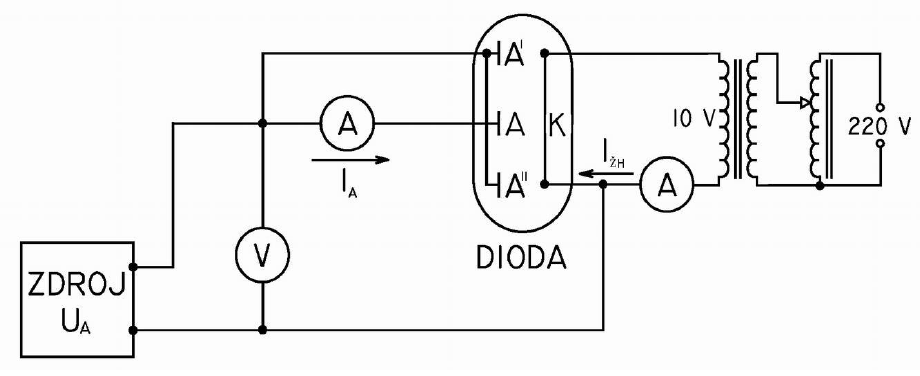
\includegraphics[width=12cm]{att/pyromet2.png}
%			\caption{Zapojení pro měření náběhového proudu. Převzato z \cite{bib:zadani}.}
%			\label{fig:s_aparatura_nasyc}
%			\end{figure}	
%			
%			\begin{figure}[h!]
%			\centering
%			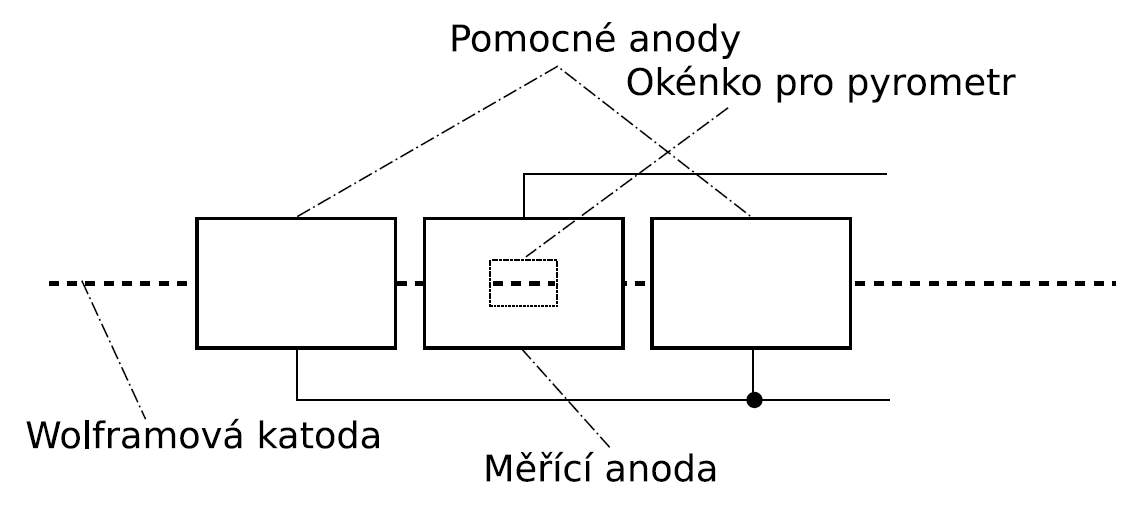
\includegraphics[width=10cm]{att/pyromet.png}
%			\caption{Geometrie uspořádání vakuové diody s pomocnými anodami pro dosažení homogenního pole. \newline Převzato z \cite{bib:zadani}.}
%			\label{fig:s_dida}
%			\end{figure}
%	
\clearpage
\section{Tabulky a grafy}


%\catcode`\-=12 % HAX na enable cline v českym bable

%%%
	\begin{figure}[h!]
	\begin{center}
	    \vspace*{-1cm}
		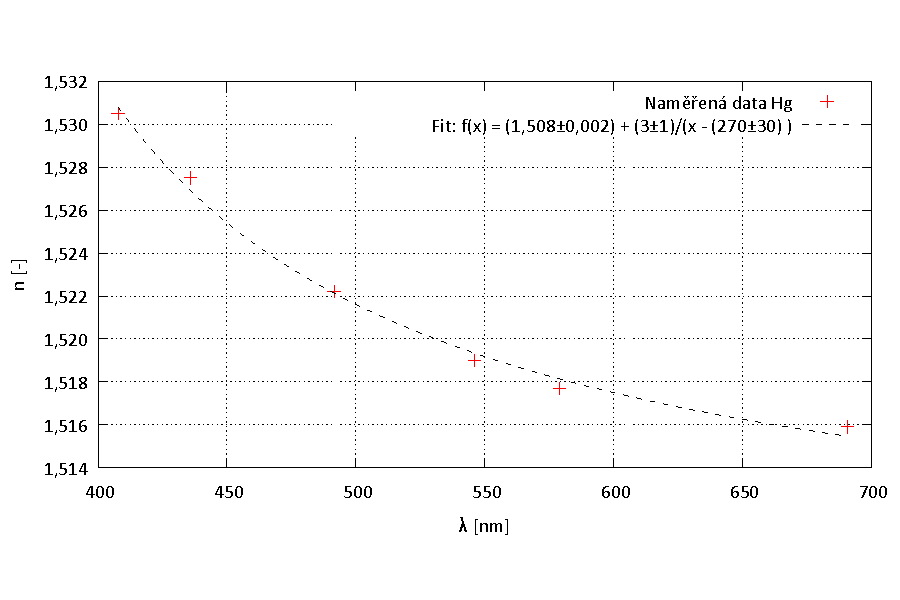
\includegraphics[width=\linewidth]{../gnuplot/hg.pdf}
	    \vspace*{-2cm}
		\caption{Závislost vypočítaného indexu lomu $n$ na teoretické vlnové délce $\lambda$ \cite{bib:na_miste}. Hodnoty jsou následně proloženy funkcí (\ref{eq:disperzni zavislost}). }
		\label{fig:g_hg}
	\end{center}
	\end{figure}
	
	\begin{figure}[h!]
	\begin{center}
	    \vspace*{-1cm}
		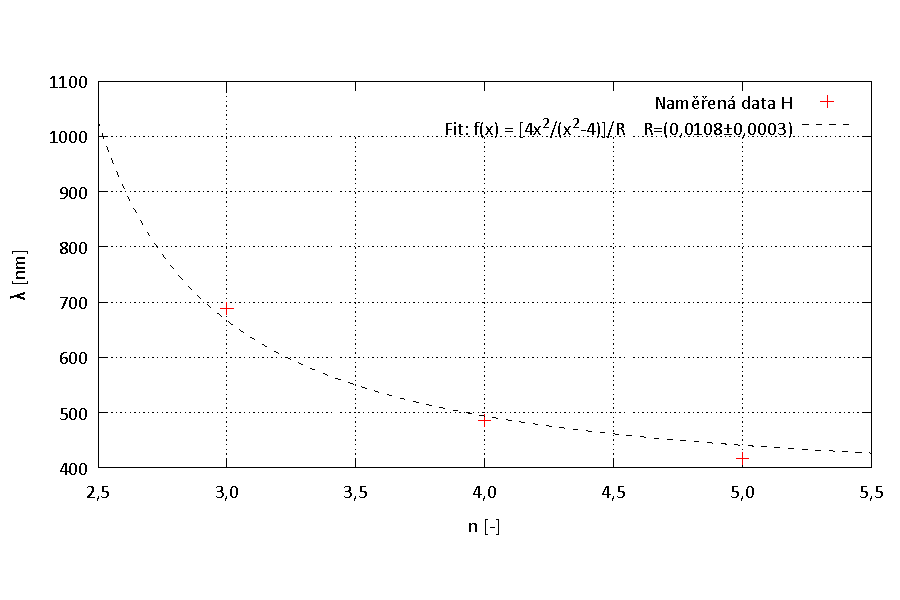
\includegraphics[width=\linewidth]{../gnuplot/r.pdf}
	    \vspace*{-2cm}
		\caption{Závislost změřené vlnové délky $\lambda$ na parametru $n$ pro spektrální čáry vodíkové výbojky. Hodnoty jsou následně proloženy funkcí (\ref{eq:balmerova serie vodik}) pro určení \emph{Rydbergovy konstanty} $R$. }
		\label{fig:g_r}
	\end{center}
	\end{figure}	
%\clearpage
				
%\clearpage
% --- Konec dokumentu --------------------------------------------------


\end{document}

